\documentclass[12pt]{article} % The document class with options

\usepackage[margin=1in]{geometry}
\usepackage[utf8]{inputenc} 
\geometry{a4paper}
\usepackage{newtxtext,newtxmath}
\usepackage[T1]{fontenc}
\usepackage{amsmath}
\usepackage{amsfonts}
\usepackage{microtype}
\usepackage{graphicx}
\usepackage{listings} % For formatting and highlighting code
\usepackage{color}    % For colors in code highlighting

% chktex-file 3
% chktex-file 8
% chktex-file 10
% chktex-file 17
% chktex-file 18
% chktex-file 36
% chktex-file 44

\begin{document}
\setlength{\parskip}{1em} 
\setlength{\parindent}{0pt}
\newcommand{\vect}[1]{\mathbf{#1}}

\begin{titlepage}  % This starts a title page environment
    \centering    % Center everything on the page

    %--- Add space at the top of the page ---
    \vspace*{2cm}
    
    %--- Title ---
    \normalsize \textbf{MEng Project Report} \\
    \vspace{0.5cm}  % Space between lines
    \normalsize\textbf{Model Analysis of DTMB5415 and BURNSI Ship Model} \\
    \vspace{2cm}  % Space between the title and the author name
    
    %--- Author ---
    \normalsize by\\
    \vspace{1cm}
    \normalsize Jincong Li \\ 
    \vspace{1cm}
    \normalsize M.Eng, The University of British Columbia, 2024
    \vspace{11cm}  % Space between the author and the date
    
    %--- Date ---
    \normalsize \today

    \vfill  % Push the following content to the bottom of the page
    %--- Bottom part of the page ---
    © Jincong Li, 2024
\end{titlepage}
\tableofcontents
\newpage
\section{Abstract}

\section{Introduction}
This project investigated into the global response of BURNSi ship model under the influence of surface waves.

\subsection{DTMB5415}

The ship model used for the first part of this project is DTMB5415, which was conceived as a preliminary design for a Navy surface combatant around 1980. The hull geometry of Model 5415 includes both a sonar dome and a transom stern. Propulsion is provided through twin open-water propellers driven by shafts supported by struts.

It is important to note that no full-scale ship exists for this model. The hull geometry and relevant loading conditions and speeds are detailed in the Appendix section.
\begin{figure}[h]
    \centering
    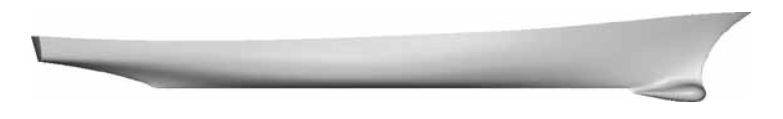
\includegraphics[width=1\textwidth]{DTMB.png}
    \caption{Side of DTMB5415}
\end{figure}


\subsection{BURNSI Ship Model}

\section{Methodology}
The main workflow of this project is first reproduce the result from section 9.2 of the Vaibhav's Ph.D thesis\cite{joshi2018}. 
Then replace the DTMB5415 ship model with the BURNSi ship model to conduct a model analysis of that ship. The main target is the
heave motion of the BURNSi ship model under the same inlet wave conditions as in the section 9.2 of \cite{joshi2018}.
\subsection{Mesh}
\begin{figure}[h]
    \centering
    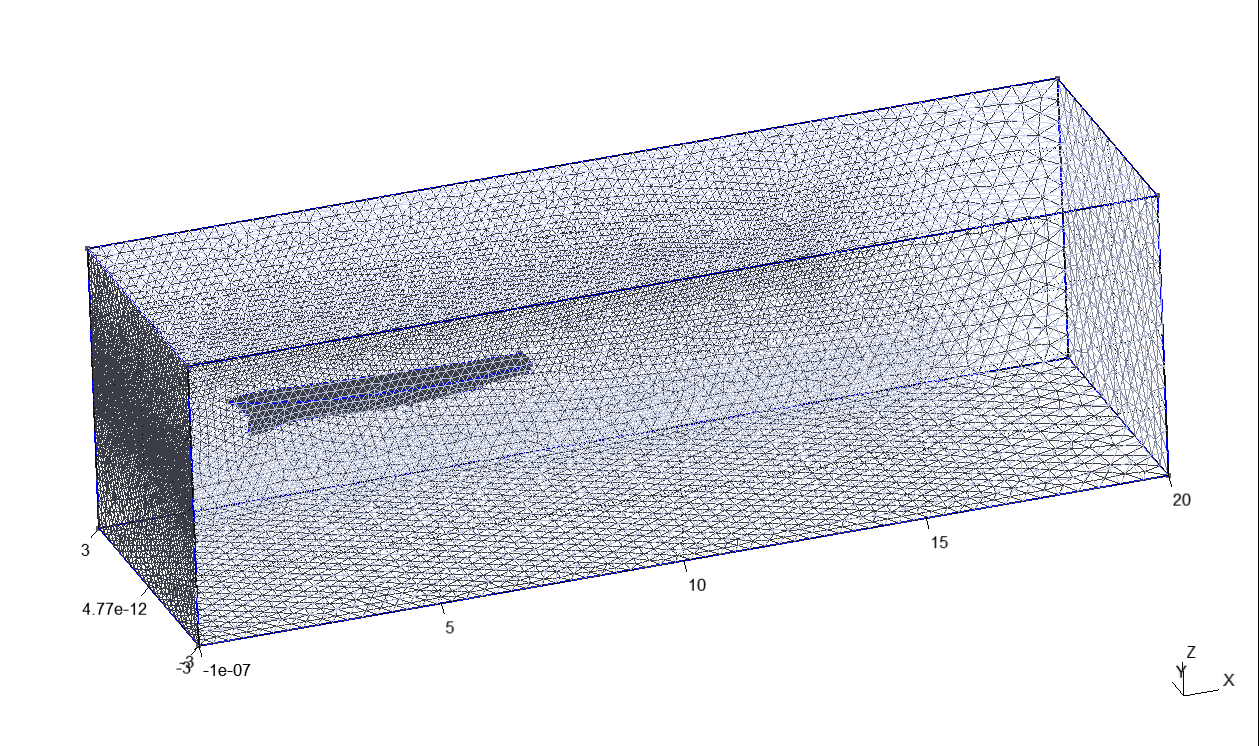
\includegraphics[width=1\textwidth]{Mesh_1.png}
    \caption{Mesh of the Domain}
    
\end{figure}
\begin{figure}[h]
    \centering
    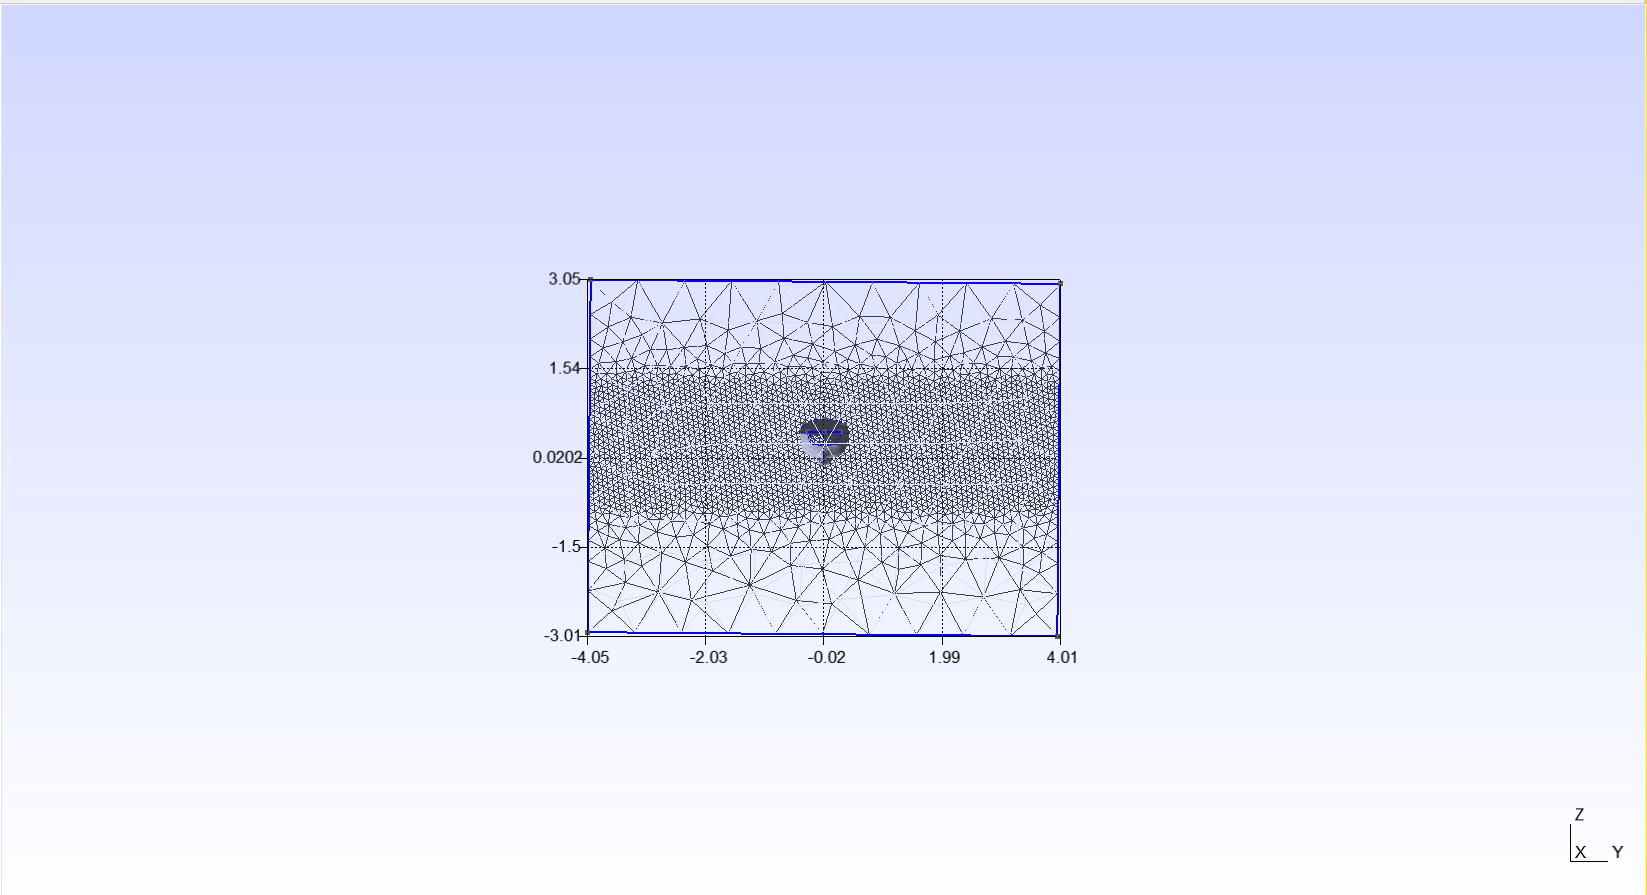
\includegraphics[width=1\textwidth]{Mesh_2.png}
    \caption{Front View of the Mesh}
\end{figure}

\begin{figure}[h]
    \centering
    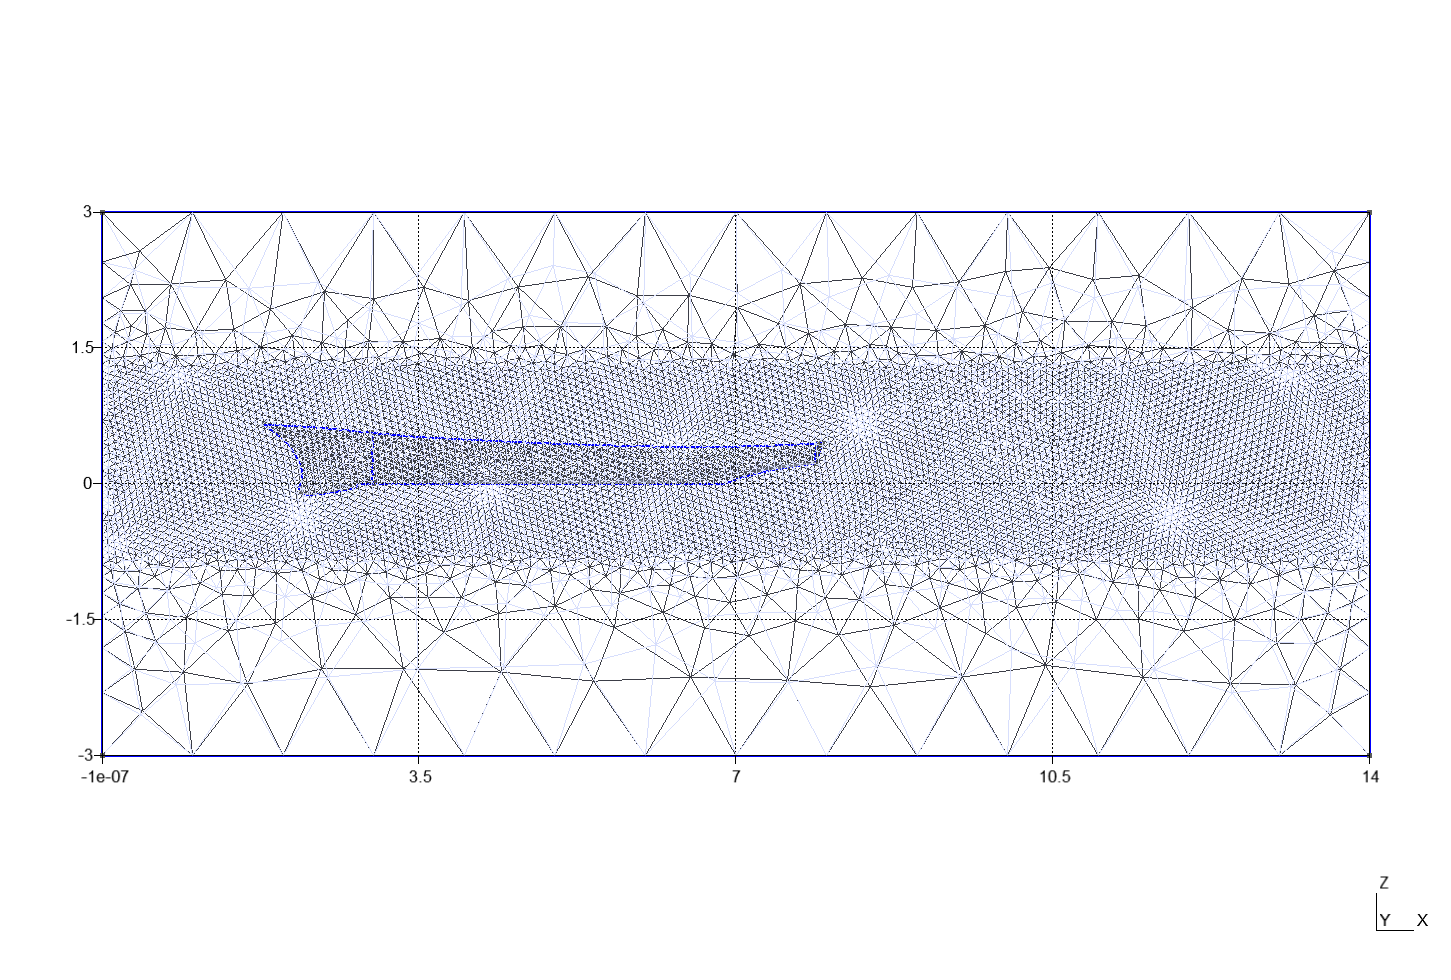
\includegraphics[width=1\textwidth]{Mesh_3.png}
    \caption{Side View of the Mesh}
\end{figure}

\begin{figure}[h]
    \centering
    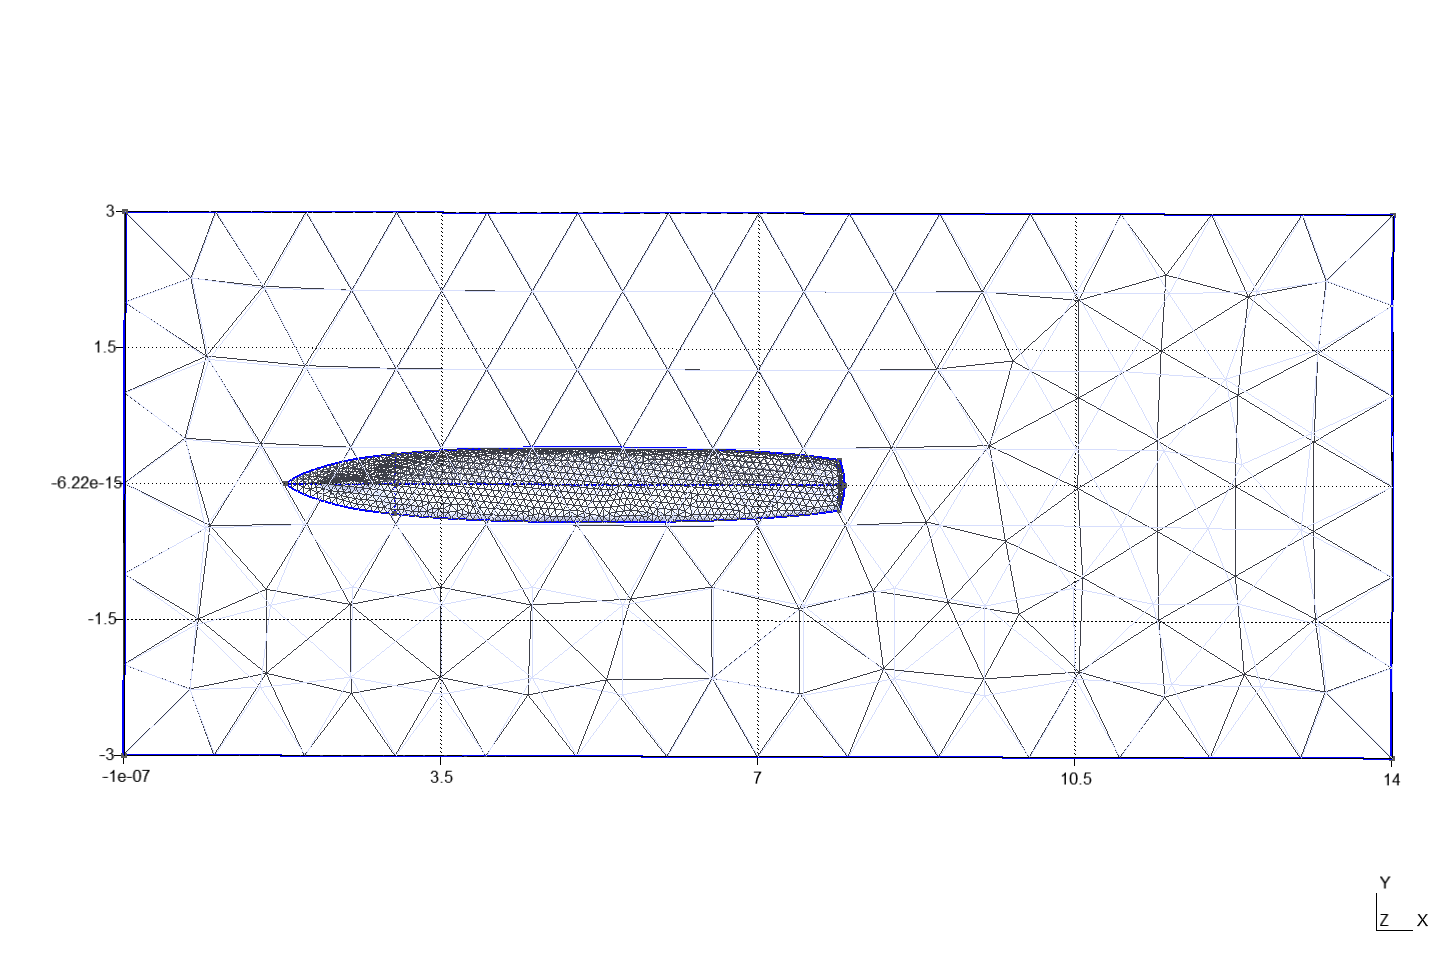
\includegraphics[width=1\textwidth]{Mesh_4.png}
    \caption{Top View of the Mesh}
\end{figure}
\clearpage
\subsection{Wave Configuration}
\begin{table}[ht]
    \caption{Wave Conditions}
    \centering
    \begin{tabular}{|c|c|c|}
        \hline
        Parameters & Value & Unit\\
        \hline   
        $H_w$ & 0.32032 & m \\
        $k_w$ & 1.0845 & m\\
        $\lambda_w$ & 0.91 & m\\
        $T_w$ & 1.929 & m \\
        \hline
    \end{tabular}
\end{table}


\section{Result}

\section{Discussion}

\section{Conclusion}



\section{Reference}
\begin{thebibliography}{99}
    \bibitem{joshi2018}
    Vaibhav Joshi, \emph{Variational Methods and Applications for Turbulent Single and Two-Phase Fluid-Structure Interaction}, ScholarBank@NUS Repository, 2018.
\end{thebibliography}

\section{Appendix}
\subsection{DTMB 5415 Specifications}
\begin{table}[h!]
    \centering
    \begin{tabular}{|c|c|c|c|c|c|}
        \hline
        & \textbf{Full-Scale} & \textbf{\textcolor{blue}{MARIN}} & \textbf{\textcolor{blue}{INSEAN}} & \textbf{\textcolor{blue}{IIHR}} &\\ \hline
        \textbf{\textcolor{blue}{Lpp (m)}} & 142.00 & 4.002 & 4.002 & 5.719 & 3.048 \\ \hline
        \textbf{\textcolor{blue}{Lwl (m)}} & 142.18 & 4.007 & 4.008 & 5.726 & 3.052 \\ \hline
        \textbf{\textcolor{blue}{Bwl (m)}} & 19.06 & 0.537 & \textcolor{green}{0.538} & 0.768 & 0.409 \\ \hline
        \textbf{\textcolor{blue}{T (m)}} & 6.15 & 0.173 & \textcolor{green}{0.172} & 0.248 & 0.132 \\ \hline
        \textbf{\textcolor{blue}{Displacement (m\(^3\))}} & 8424.4 & 0.189 & \textcolor{green}{0.188} & 0.554 & 0.0826 \\ \hline
        \textbf{\textcolor{blue}{S w/o rudder (m\(^2\))}} & 2972.6 & 2.361 & \textcolor{green}{2.424} & TBD & TBD \\ \hline
        \textbf{\textcolor{blue}{CB}} & 0.507 & 0.507 & 0.507 & 0.506 & TBD \\ \hline
        \textbf{\textcolor{blue}{CM}} & 0.821 & 0.821 & 0.821 & 0.821 & 0.821 \\ \hline
        \textbf{\textcolor{blue}{LCB (\%Lpp), fwd+}} & -0.683 & -0.683 & \textcolor{green}{-0.652} & \textcolor{green}{-0.652} & TBD \\ \hline
    \end{tabular}
    \caption{Main particulars of the ship model}
    \label{tab:main_particulars}
\end{table}


\end{document}